\documentclass[12pt]{article}

\usepackage{sbc-template}
\usepackage{graphicx,url}
\usepackage[utf8]{inputenc}
\usepackage[brazil]{babel}

\sloppy

\title{COMPARAÇÃO DA EFICIÊNCIA DE CNNS NA CLASSIFICAÇÃO DE DOENÇAS EM PLANTAS}

% \author{Angelo Gabriel\inst{1}, Vinicius Tessele\inst{1},\\
% Claudio Honorio da Silva Junior\inst{1}, Leonardo Tampelini\inst{1}}

% \address{Departamento de Inteligência Artificial, Biopark Educação -- Toledo, PR, Brasil
% \email{\{angelo.gabriel, vinicius.tessele, claudio.silva, leonardo.tampelini\}@bioparkedu.com.br}
% }

\begin{document}

\maketitle

\begin{abstract}
This study investigates the effectiveness of three consolidated Convolutional Neural Network (CNN) architectures for plant disease classification using the PlantVillage dataset. The evaluated models include InceptionV3, ResNet50, and VGG16, all utilizing transfer learning with pre-trained ImageNet weights. Automated plant disease detection is a key component of precision agriculture, contributing to reduced crop losses and production costs. While traditionally performed by specialists, the adoption of artificial intelligence-based solutions can provide efficient support for decision-making in the field. The study describes the image preprocessing steps, including resizing to 224x224 pixels, normalization, dataset splitting into training, validation, and testing sets, and the application of data augmentation techniques. The models were evaluated using accuracy, precision, recall, F1-score, and confusion matrix. The results enable the identification of the most efficient architecture in terms of performance and computational feasibility for the development of automated agricultural monitoring systems. 
\textbf{keywords:} Artificial Neural Networks, Disease Classification, Deep Learning, Transfer Learning.
\end{abstract}

\renewcommand{\abstractname}{Resumo}

\begin{abstract}
Este estudo apresenta a implementação e comparação da eficiência de três arquiteturas consolidadas de Redes Neurais Convolucionais (CNNs) pré-treinadas: InceptionV3, ResNet50 e VGG16, na tarefa de classificação de doenças em plantas utilizando o conjunto de dados PlantVillage. Todas as arquiteturas utilizaram transfer learning com pesos pré-treinados do ImageNet. A detecção automatizada de doenças em plantas é essencial para a agricultura moderna, assegurando a redução das perdas e dos custos de produção. A detecção e classificação de doenças são feitas por profissionais qualificados, entretanto, a incorporação de novas tecnologias pode oferecer suporte adicional a esses profissionais. A inteligência artificial, presente no dia a dia, pode ser integrada como solução baseada em IA para apoiar esses profissionais na tomada de decisão. O uso de Redes Neurais Artificiais Convolucionais, as conhecidas CNNs, passa a ser fundamental, com alta precisão. O trabalho detalha as etapas de pré-processamento de dados, incluindo redimensionamento para 224x224 pixels, normalização, divisão em conjuntos de treino, validação e teste, e aplicação de técnicas de aumento de dados. Os modelos foram treinados e avaliados utilizando métricas como acurácia, precisão, recall, F1-score e matriz de confusão. Os resultados práticos da implementação permitem identificar a arquitetura mais adequada em termos de desempenho e eficiência computacional para o desenvolvimento de sistemas automatizados de monitoramento agrícola.  
\textbf{Palavras-chave:} Redes Neurais Artificiais, Classificação de Doenças, Aprendizado Profundo, Transfer Learning. 
\end{abstract}

\section{Introdução} 
A agricultura sempre enfrenta desafios para garantir a segurança alimentar, são diversas ameaças, que são desde intempéries do clima quando ameaças de pragas e doenças. Essas ocorrências podem levar a perdas significativas na produção agrícola, impactando diretamente a economia e a subsistência de comunidades. Segundo \cite{tessele2024treinamento}, o uso de redes neurais artificiais pode otimizar a tomada de decisões no campo, contribuindo para identificar o momento ideal de manejo, como a dessecação da soja, com maior precisão e menor subjetividade. Métodos tradicionais de identificação de doenças, geralmente realizados por especialistas, por vezes são lentos e caros e suscetíveis a erros, especialmente em grandes extensões de cultivo. A necessidade de soluções mais rápidas, precisas e escaláveis impulsiona a busca por tecnologias inovadoras envolvendo a inteligência artificial (IA).  

A IA atualmente é ferramenta presente no cotidiano das pessoas \cite{garcia2020etica}, e na agricultura vem se fortalecendo e é crescente o uso da tecnologia baseada em IA em todas as fases do cultivo \cite{vicari2021influencias}. A utilização da inteligência artificial no processo de tomada de decisões torna-se cada vez mais relevante, sendo necessário considerar aspectos de accountability e transparência \cite{pinto2020utilizacao}. Dentro do grande guarda-chuva que é a IA, o estudo aborda o uso das Redes Neurais Convolucionais (CNNs) como uma ferramenta poderosa e transformadora. As CNNs, uma subclasse do aprendizado profundo, são particularmente eficazes para tarefas de visão computacional, como reconhecimento e classificação de imagens \cite{simeon2008aplicacao}. Sua capacidade de aprender automaticamente características hierárquicas a partir dos dados de entrada, eliminando a necessidade de engenharia manual de atributos, as torna ideais para a análise de imagens de plantas. De acordo com \cite{mohanty2016deep}, técnicas baseadas em deep learning, especialmente CNNs, mostraram resultados promissores na identificação automática de doenças em folhas com alta acurácia. Modelos como VGGNet, ResNet, Inception e EfficientNet têm demonstrado sucesso notável em diversas aplicações, incluindo a detecção e classificação de doenças em folhas e outras partes de plantas, oferecendo uma abordagem automatizada e de alta precisão.  

O dataset PlantVillage é amplamente utilizado na comunidade de pesquisa em visão computacional, servindo como base fundamental para o treinamento e a avaliação de modelos de classificação de doenças em plantas. \cite{hughes2015open} introduziram o PlantVillage como um repositório público contendo várias imagens de folhas com doenças, com o intuito de apoiar a comunidade científica na criação de soluções automatizadas de detecção e diagnóstico. Contendo uma vasta coleção de imagens de folhas de diversas espécies, categorizadas entre plantas saudáveis e com diferentes tipos de doenças, ele proporciona um ambiente robusto para o desenvolvimento e teste de algoritmos. A diversidade das imagens neste dataset, que abrange variações de iluminação, ângulos e estágios de doença, permite o desenvolvimento de modelos com boa capacidade de generalização para cenários do mundo real. Tais estudos são fundamentais para que possam ser explorados os melhores modelos para cada cenário. A aplicação de técnicas de inteligência artificial para testagem e desenvolvimento de software tem se mostrado promissora \cite{sales2020analise}, assim como a utilização dessas técnicas em sistemas de manutenção baseada em condição \cite{simeon2008aplicacao}. Nem sempre um modelo se adequa à qualidade das imagens do conjunto de dados para treinamento e teste, por isso é importante comparar os resultados e aprimorar o seu aprendizado.  

Este estudo tem como objetivo principal a implementação e comparação da eficiência de três arquiteturas consolidadas de CNNs pré-treinadas: InceptionV3, ResNet50 e VGG16. A escolha dessas arquiteturas reflete diferentes abordagens arquiteturais no design de redes neurais profundas: a InceptionV3 com sua arquitetura modular e uso eficiente de recursos computacionais através de módulos Inception; a ResNet50 com seus blocos residuais que permitem o treinamento de redes mais profundas ao mitigar o problema de desaparecimento de gradientes; e a VGG16 com sua arquitetura linear e camadas convolucionais densas que estabeleceu fundamentos importantes para CNNs modernas. Todas as arquiteturas serão utilizadas com transfer learning, aproveitando pesos pré-treinados no ImageNet e adaptando-as para o domínio específico de classificação de doenças em plantas.

A comparação será realizada em termos de métricas de desempenho como acurácia, precisão, recall, F1-score e análise da matriz de confusão, além de considerar a eficiência computacional, como tempo de treinamento. \cite{tessele2024modelo} destacam que a análise comparativa de diferentes arquiteturas é essencial, pois a acurácia geral pode mascarar erros graves, especialmente quando há classes semelhantes. 

Ao final, espera-se não apenas fornecer uma análise comparativa aprofundada do desempenho dessas três arquiteturas consolidadas no contexto da classificação de doenças em plantas, mas também oferecer insights práticos para a seleção da arquitetura mais adequada para o desenvolvimento de sistemas de monitoramento agrícola eficientes e robustos. O entendimento dessas abordagens é fundamental para o desenvolvimento de sistemas de inteligência artificial em cursos de tecnologia, alinhando a formação acadêmica com as demandas do mercado e as tendências de IA \cite{vicari2021influencias}.

\section{METODOLOGIA / MATERIAIS E MÉTODOS} 
A metodologia deste estudo é centrada na implementação, treinamento e avaliação prática de diferentes arquiteturas de Redes Neurais Convolucionais (CNNs) para a classificação de doenças em plantas. O processo será dividido em três fases principais: Preparação dos Dados, Treinamento dos Modelos e Avaliação do Desempenho. 
\subsection{Preparação dos Dados}
Para esta pesquisa, o conjunto de dados PlantVillage foi utilizado \cite{hughes2015open}, contendo imagens de folhas de diversas espécies, rotuladas quanto à presença e tipo de doença, ou status saudável. As etapas de preparação dos dados seguiram as boas práticas de aprendizado profundo, implementadas utilizando a biblioteca Keras no Python: 
\subsubsection*{Carregamento e Redimensionamento das Imagens}
As imagens do dataset foram carregadas e redimensionadas para um padrão de 224x224 pixels, utilizando image\_dataset\_from\_directory.Esse tamanho é comumente utilizado e otimizado para as arquiteturas de CNN pré-treinadas. 
\subsubsection*{Normalização}
Os valores dos pixels das imagens foram normalizados para a faixa de [0, 1] automaticamente pelo pipeline de pré-processamento. Isso otimiza o processo de treinamento, ajudando na convergência dos algoritmos de otimização. 
\subsubsection*{Divisão dos Dados}
O dataset foi dividido em conjuntos de treinamento, validação e teste nas proporções de aproximadamente 80\%, 10\% e 10\%, respectivamente, configurados no image\_dataset\_from\_directory para garantir a separação adequada para treinamento e avaliação. 
\subsubsection*{Aumento de Dados (Data Augmentation)}
Para aumentar a robustez e capacidade de generalização dos modelos, técnicas de aumento de dados foram aplicadas ao conjunto de treinamento. Isso foi realizado através da camada RandomFlip("horizontal\_and\_vertical"), RandomRotation(0.2), RandomZoom(0.2), RandomContrast(0.2) e RandomTranslation(height\_factor=0.2, width\_factor=0.2) do Keras. Esta etapa visou criar variações sintéticas das imagens originais e prevenir o overfitting. 
\subsection{Treinamento dos Modelos}
Três arquiteturas de CNNs pré-treinadas foram implementadas e treinadas de forma comparativa, conforme especificado no notebook: 
\subsubsection*{InceptionV3}
A arquitetura InceptionV3 foi carregada com pesos pré-treinados do ImageNet (weights='imagenet'). Após a remoção da camada de classificação original, uma nova camada GlobalAveragePooling2D foi adicionada, seguida de uma camada Dense para as 38 classes de saída com ativação softmax. As camadas convolucionais pré-treinadas da InceptionV3 foram congeladas no início e então algumas camadas superiores foram descongeladas para permitir o fine-tuning. 
\subsubsection*{ResNet50}
A arquitetura ResNet50 foi utilizada, carregada com pesos pré-treinados do ImageNet (weights='imagenet'). A camada de classificação original foi substituída por uma nova camada Dense com ativação softmax, adaptada para as 38 classes de doenças/estados saudáveis do PlantVillage. As camadas convolucionais pré-treinadas da ResNet50 foram congeladas para feature extraction, focando o treinamento apenas na nova camada de classificação, e em seguida, parte das camadas do backbone foi descongelada para fine-tuning de forma a ajustar melhor o modelo aos dados específicos.
\subsubsection*{VGG16}
Similarmente, a arquitetura VGG16 foi carregada com pesos pré-treinados do ImageNet (weights='imagenet'). A camada de classificação foi removida e substituída por uma nova camada Dense para as 38 classes, seguida de uma ativação softmax. O backbone da VGG16 foi congelado para transferir o aprendizado, e posteriormente, uma parte foi descongelada para fine-tuning. 

O treinamento de cada modelo, realizado com apenas uma CPU Intel Core i5-10300H, incluiu a definição e ajuste de hiperparâmetros, como taxa de aprendizado, número de épocas e tamanho do lote. 

O otimizador tf.keras.optimizers.Adam foi utilizado, e a função de perda tf.keras.losses.CategoricalCrossentropy foi selecionada, apropriada para problemas de classificação multiclasse. Callbacks como EarlyStopping (monitorando val\_loss para interromper o treinamento quando a validação não melhora) e ReduceLROnPlateau (monitorando val\_loss para reduzir a taxa de aprendizado quando o desempenho não melhora) foram utilizados para otimizar o processo de treinamento e evitar overfitting. 

\subsection{Avaliação do Desempenho}
Após o treinamento, o desempenho de cada modelo foi rigorosamente avaliado usando o conjunto de dados de teste, que não foi visto durante o treinamento. As métricas de avaliação incluíram: 
\subsubsection*{Acurácia}
Medida geral de quão bem o modelo classifica as imagens corretamente.
\subsubsection*{Precisão (Precision)}
A proporção de identificações positivas corretas (verdadeiros positivos) em relação ao total de identificações positivas (verdadeiros positivos + falsos positivos). 
\subsubsection*{Recall (Sensibilidade)}
A proporção de identificações positivas corretas (verdadeiros positivos) em relação ao total de casos positivos reais (verdadeiros positivos + falsos negativos). 
\subsubsection*{F1-Score}
A média harmônica da precisão e do recall, oferecendo um equilíbrio entre as duas. 
\subsubsection*{Matriz de Confusão}
    Uma ferramenta visual que detalha o número de verdadeiros positivos, verdadeiros negativos, falsos positivos e falsos negativos para cada modelo, fornecendo uma visão granular de seu desempenho. As matrizes de confusão (absoluta e percentual) foram geradas e visualizadas usando seaborn.heatmap. 

Além das métricas quantitativas, será realizada uma análise qualitativa das previsões dos modelos, identificando os tipos de erros e os desafios específicos enfrentados por cada arquitetura. A eficiência computacional será avaliada monitorando o tempo de treinamento e inferência em um ambiente controlado (CPU ou GPU, conforme disponível no ambiente de execução do notebook). 

\subsection{Análise Comparativa}
Após a avaliação dos modelos, uma análise comparativa será realizada levando em consideração os seguintes critérios:
\subsubsection*{Desempenho de classificação}
A acurácia, precisão, recall e F1-score serão comparados entre os modelos. 
\subsubsection*{Eficiência computacional}
O tempo de treinamento e inferência de cada modelo será medido para avaliar o uso de recursos computacionais, como memória e tempo de processamento.  
\subsubsection*{Capacidade de generalização}
Será comparado o desempenho de cada modelo no conjunto de validação e teste, a fim de verificar sua capacidade de generalizar para dados não vistos durante o treinamento. 

\section{Resultados}
Esta seção apresenta os resultados obtidos com o treinamento e a avaliação dos três modelos de CNNs pré-treinadas: InceptionV3, ResNet50 e VGG16. O treinamento foi conduzido por 3 épocas para cada modelo, utilizando o dataset PlantVillage \cite{hughes2015open}, e os resultados são sumarizados a seguir, com gráficos de acurácia e perda (treinamento e validação) e matrizes de confusão detalhadas. 
\begin{figure}[!ht]
\centering
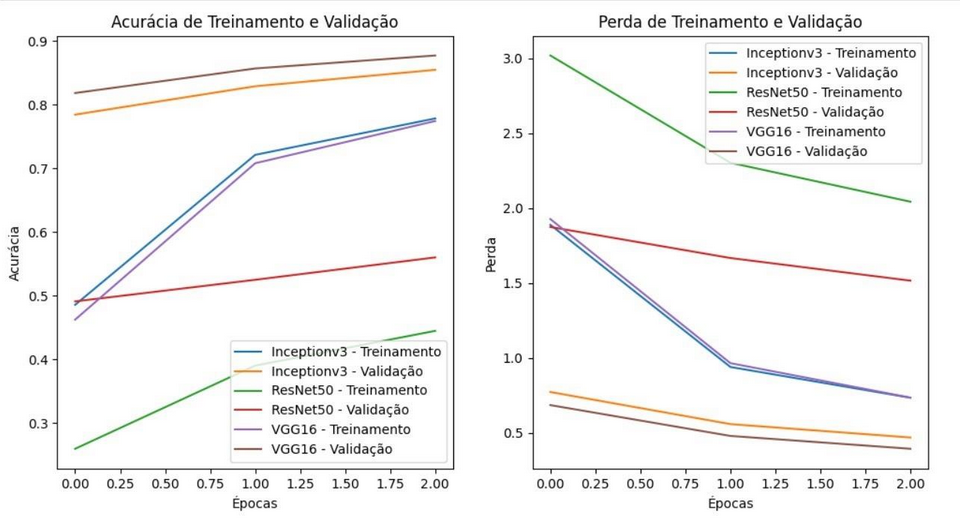
\includegraphics[width=5.5in]{figs/fig001.png}
\caption{Curvas de Acurácia e Perda para o Modelo InceptionV3, ResNet50 e VGG16, Fonte: Autoria própria (2025). }
\label{fig:fig01}
\end{figure}
A Figura\ref{fig:fig01} exibe, de forma comparativa, as curvas de acurácia e perda para os conjuntos de treinamento e validação dos três modelos ao longo das épocas. Essas curvas permitem visualizar a evolução do desempenho de cada rede durante o processo de aprendizagem, bem como identificar possíveis indícios de overfitting ou subajuste. 
\subsection{Desempenho do Modelo InceptionV3}
O treinamento do modelo InceptionV3 demonstrou uma rápida convergência e alta performance. Os gráficos de acurácia e perda durante o treinamento e validação são apresentados na Figura\ref{fig:fig01}. 
A acurácia final de validação para o InceptionV3 atingiu 0.8538, com uma perda de validação de 0.4623. Durante as épocas iniciais, observou-se uma acurácia de treinamento de aproximadamente 0.8832 e uma perda de 0.3754. O tempo de treinamento por época foi de aproximadamente 1500-1700 segundos. A matriz de confusão detalhada para o InceptionV3, que ilustra o desempenho do modelo em cada classe, é apresentada na Figura\ref{fig:fig02}. 
\begin{figure}[!ht]
\centering
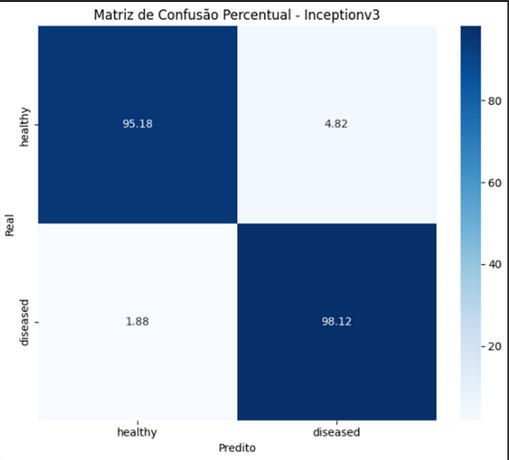
\includegraphics[width=3.5in]{figs/fig002.png}
\caption{Matriz de Confusão para o Modelo InceptionV3, Fonte: Autoria própria (2025).}
\label{fig:fig02}
\end{figure}
\subsection{Desempenho do Modelo ResNet50 }
O modelo ResNet50 também foi treinado e avaliado, com suas curvas de acurácia e perda durante o processo de treinamento e validação ilustradas na Figura\ref{fig:fig01}. 
A acurácia final de validação para o ResNet50 foi de 0.5650, com uma perda de validação de 1.5099. A acurácia de treinamento ao final das 3 épocas foi de aproximadamente 0.5629, e a perda de 1.5361. Este modelo apresentou um tempo de treinamento por época em torno de 2500-2600 segundos. A matriz de confusão correspondente ao desempenho do ResNet50 é exibida na Figura\ref{fig:fig03}. 
\begin{figure}[!ht]
\centering
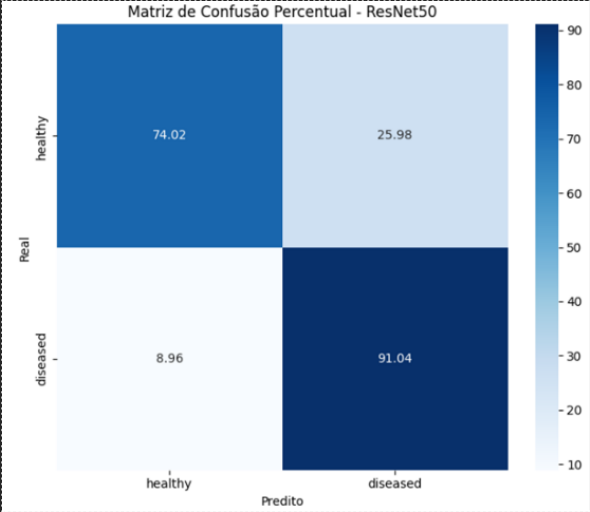
\includegraphics[width=3.5in]{figs/fig003.png}
\caption{Matriz de Confusão para o Modelo ResNet50, Autoria própria (2025).}
\label{fig:fig03}
\end{figure}
\subsection{Desempenho do Modelo VGG16 }
Os resultados do treinamento do modelo VGG16, incluindo as curvas de acurácia e perda para os conjuntos de treinamento e validação, são apresentados na Figura\ref{fig:fig01}. 

 O modelo VGG16 alcançou uma acurácia final de validação de 0.8809, com uma perda de validação de 0.3936. A acurácia de treinamento ao final das 3 épocas foi de aproximadamente 0.9130, e a perda de 0.3012. O tempo de treinamento por época foi significativamente maior, aproximadamente 5800 segundos. A matriz de confusão que detalha o desempenho de classificação do VGG16 é mostrada na Figura\ref{fig:fig04}. 
\begin{figure}[!ht]
\centering
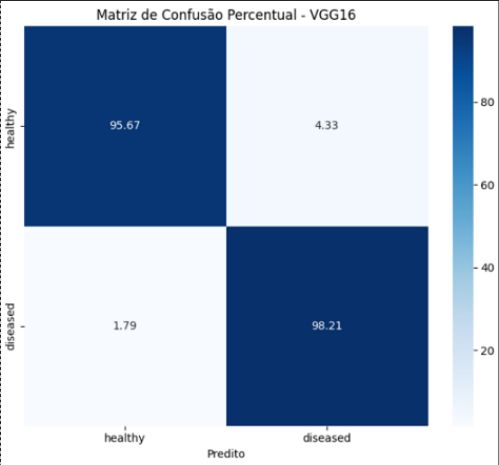
\includegraphics[width=3.5in]{figs/fig004.png}
\caption{Matriz de Confusão para o Modelo VGG16, Fonte: Autoria própria (2025).}
\label{fig:fig04}
\end{figure}
\subsection{DISCUSSÃO}
A análise dos resultados obtidos com o treinamento e avaliação das arquiteturas InceptionV3, ResNet50 e VGG16 no dataset PlantVillage \cite{hughes2015open} revela importantes insights sobre a eficácia de CNNs pré-treinadas na classificação de doenças em plantas. Conforme demonstrado no gráfico de acurácia e perda (Figura \ref{fig:fig01}) e nas matrizes de confusão (Figuras \ref{fig:fig02}, \ref{fig:fig03} e \ref{fig:fig04}) apresentados na seção de Resultados, os modelos VGG16 e InceptionV3 alcançaram desempenho notável, com acurácias de validação consistentemente elevadas. 

Observando os resultados, a arquitetura VGG16 (Figura \ref{fig:fig04}) demonstrou o maior valor de acurácia de validação final (0.8809) dentre os modelos treinados, indicando sua forte capacidade de aprendizado e generalização para o conjunto de dados. Contudo, esse desempenho veio acompanhado de um tempo de treinamento por época significativamente maior (aproximadamente 5800 segundos), o que é esperado dada a sua arquitetura com um grande número de parâmetros e camadas convolucionais densas. 

A InceptionV3 (Figura \ref{fig:fig02}) também exibiu um desempenho robusto, com uma acurácia de validação final de 0.8538. Embora ligeiramente inferior à VGG16 em acurácia, a InceptionV3 se destaca por sua eficiência computacional, apresentando um tempo de treinamento por época consideravelmente menor (aproximadamente 1500-1700 segundos). Isso se deve à sua arquitetura modular, que utiliza diferentes tamanhos de filtros em paralelo e emprega técnicas de redução de dimensionalidade para otimizar o uso de recursos, tornando-a uma opção atraente para cenários onde a velocidade de treinamento e inferência é crucial. A matriz de confusão da InceptionV3 revela uma alta precisão e recall para a maioria das classes, indicando sua eficácia na distinção entre diferentes condições de saúde das plantas, conforme observado por \cite{mohanty2016deep} em estudos similares. 

Em contraste, o modelo ResNet50 (Figura \ref{fig:fig03}) apresentou uma acurácia de validação final consideravelmente mais baixa (0.5650) em comparação com a VGG16 e a InceptionV3. Este resultado, juntamente com uma perda de validação mais alta (1.5099), sugere que a configuração de treinamento aplicada (apenas 3 épocas e fine-tuning talvez não tão extensivo) pode não ter sido suficiente para que o ResNet50, com sua complexidade de blocos residuais, explorasse todo o seu potencial neste dataset. A ResNet50 é conhecida por sua capacidade de treinar redes muito profundas e mitigar o problema do desaparecimento de gradientes, mas pode exigir mais épocas ou um ajuste mais fino dos hiperparâmetros e das camadas a serem descongeladas para superar as outras arquiteturas em cenários específicos. Uma limitação significativa deste estudo é o treinamento limitado a apenas 3 épocas, o que pode ser insuficiente para permitir que modelos mais complexos, como a ResNet50, alcancem sua convergência ideal. O tempo de treinamento por época (2500-2600 segundos) foi intermediário entre VGG16 e InceptionV3. 

A alta acurácia alcançada pela VGG16 e InceptionV3, aliada à baixa incidência de falsos positivos e negativos observados em suas matrizes de confusão, indica o potencial dessas arquiteturas para serem integradas em sistemas de apoio à decisão para agricultores, como demonstrado por \cite{tessele2024modelo} em aplicações similares com ML.NET. Um diagnóstico precoce e preciso de doenças pode diminuir as perdas na produção e otimizar os custos. A escolha da arquitetura ideal em uma aplicação prática dependerá de um equilíbrio entre o desempenho desejado e a eficiência computacional. Para implantações em dispositivos móveis ou sistemas embarcados em drones e equipamentos agrícolas, a InceptionV3 pode ser mais vantajosa devido ao seu tempo de treinamento e inferência mais rápidos, mesmo que a VGG16 possa oferecer uma acurácia marginalmente superior. 

\subsubsection*{Limitações do Estudo}
Este estudo apresenta algumas limitações importantes que devem ser consideradas na interpretação dos resultados. Primeiramente, o treinamento limitado a apenas 3 épocas pode ter impactado significativamente o desempenho dos modelos, especialmente da ResNet50, que historicamente requer mais iterações para convergir adequadamente. Esta limitação temporal pode explicar parcialmente a performance inferior da ResNet50 em comparação com VGG16 e InceptionV3.

Adicionalmente, a dependência da qualidade e representatividade do dataset PlantVillage deve ser considerada; variações regionais de doenças, condições de iluminação extremas e diferentes estágios de desenvolvimento da planta podem não estar totalmente representados, o que pode impactar a generalização dos modelos para cenários do mundo real não vistos. A ausência de análise de classes desbalanceadas também representa uma limitação, pois o desbalanceamento pode mascarar problemas de performance em classes minoritárias, conforme destacado por \cite{tessele2024modelo}.

Finalmente, a avaliação da eficiência computacional foi limitada ao tempo de treinamento, não incluindo métricas como consumo de memória RAM/VRAM, tempo de inferência com batches realistas, ou análise de FLOPs (operações de ponto flutuante), que seriam relevantes para aplicações práticas em sistemas embarcados ou dispositivos móveis.

\subsubsection*{Trabalhos Futuros}
Para futuras pesquisas, sugere-se a exploração de outras arquiteturas de CNNs, como EfficientNet ou Vision Transformers (ViT), que têm demonstrado resultados promissores em tarefas de classificação de imagens. O aumento do número de épocas de treinamento, especialmente para modelos mais complexos como ResNet50, pode revelar seu verdadeiro potencial. A incorporação de técnicas de aumento de dados mais avançadas, como mixup, cutmix ou AutoAugment, pode enriquecer ainda mais o conjunto de treinamento e melhorar a robustez dos modelos.

A implementação de análises mais detalhadas sobre o balanceamento de classes e o impacto de possíveis desbalanceamentos na performance dos modelos seria valiosa. Além disso, a avaliação de métricas de eficiência computacional mais abrangentes, incluindo tempo de inferência, consumo de memória e análise de FLOPs, proporcionaria insights mais práticos para implementações reais.

Finalmente, a validação dos modelos em datasets de campo, sob condições variadas e com dados coletados em diferentes regiões geográficas, e a integração com sistemas embarcados para testes em tempo real representam direções promissoras para pesquisas futuras, contribuindo para a transição da pesquisa acadêmica para aplicações práticas na agricultura de precisão.

\section{Conclusão}
Este estudo apresentou uma análise comparativa de três arquiteturas consolidadas de CNNs pré-treinadas - InceptionV3, ResNet50 e VGG16 - para classificação de doenças em plantas utilizando o dataset PlantVillage. Os resultados demonstraram que tanto a VGG16 quanto a InceptionV3 alcançaram desempenho robusto, com acurácias de validação de 0.8809 e 0.8538, respectivamente, enquanto a ResNet50 apresentou performance inferior (0.5650), possivelmente devido à limitação de apenas 3 épocas de treinamento.

A VGG16 destacou-se pela maior acurácia, porém com maior custo computacional (5800 segundos por época), enquanto a InceptionV3 ofereceu um equilíbrio interessante entre desempenho e eficiência (1500-1700 segundos por época). Estes resultados evidenciam o potencial das CNNs pré-treinadas com transfer learning para aplicações agrícolas, contribuindo para o desenvolvimento de sistemas automatizados de monitoramento de culturas.

Para aplicações práticas, recomenda-se a InceptionV3 quando a eficiência computacional for prioritária, especialmente em dispositivos móveis ou sistemas embarcados, enquanto a VGG16 pode ser preferível quando a máxima acurácia for o critério principal. O estudo contribui para a literatura científica ao fornecer insights práticos sobre a seleção de arquiteturas CNN para agricultura de precisão, alinhando-se com as tendências atuais de integração de IA em sistemas agrícolas.

\bibliographystyle{sbc}
\bibliography{referencias}

\end{document}